% SD4H 2026 (ICML workshop) submission — 4 pages, double-blind.
%
% Build: pdflatex main && bibtex main && pdflatex main && pdflatex main
% Requires: icml2026.sty (download from the ICML 2026 site)
%
% Placeholders marked [TBD: ...] must be filled once the pilot run completes.

\documentclass{article}

% === ICML 2026 style ==========================================================
% Swap this for \usepackage[accepted]{icml2026} only on acceptance.
\usepackage{icml2026}
% If the official style isn't available yet, uncomment the fallback below:
% \usepackage[accepted]{icml2024}

\usepackage{booktabs}
\usepackage{graphicx}
\usepackage{microtype}
\usepackage{amsmath, amssymb}
\usepackage{tikz}
\usepackage{url}
\usepackage{xcolor}
\usetikzlibrary{arrows.meta,fit,positioning}
\newcommand{\tbd}[1]{\textcolor{red}{[TBD: #1]}}

% === Anonymized submission ====================================================
\icmltitlerunning{Training for Humility: LoRA Distillation of Epistemic Wrappers}

\begin{document}

\twocolumn[
\icmltitle{Training for Humility:\\
           Distilling Epistemic Wrappers into Clinical LLM Weights via LoRA}

% Leave author block blank for blind submission. Reviewers see only the
% anonymous paper + anonymized code mirror.
\icmlsetsymbol{equal}{*}
\begin{icmlauthorlist}
\icmlauthor{Anonymous Authors}{anon}
\end{icmlauthorlist}
\icmlaffiliation{anon}{Anonymous Institution}
\icmlcorrespondingauthor{Anonymous}{anonymous@example.com}
\icmlkeywords{LoRA, clinical LLMs, calibration, epistemic humility}
\vskip 0.3in
]

\printAffiliationsAndNotice{}

% =============================================================================
\begin{abstract}
Large language models deployed in medical settings exhibit an
\emph{inverted-U of failure}: accuracy collapses at both ends of case
difficulty, with the most dangerous errors concentrated on emergent
presentations where overconfident misjudgment is most harmful.
Prompt-engineered \emph{epistemic wrappers} can mitigate this at inference
time, but add latency, cost, and brittleness. We ask whether the
virtues a wrapper enforces---humility, calibration, and abstention---can
be internalized into a model's weights so that they persist
\emph{without} the wrapper at serve time. We present a pipeline for
doing so: generate wrapper-conditioned traces on
HealthBench~\cite{arora2025healthbench}, grade them against the
benchmark's per-criterion rubric, filter by score, and supervise-fine-tune
a LoRA adapter~\cite{hu2021lora} on the filtered traces. We evaluate on a
200-prompt HealthBench Hard holdout along four configurations (base and
LoRA, each with and without the wrapper) and introduce a
\emph{stratified} reporting protocol inspired by a recent Nature
Medicine triage study~\cite{natmed2026triage} that surfaces the
U of failure along difficulty and theme axes. \tbd{headline numbers
once the pilot run completes}. Code is available at an anonymized
mirror.\footnote{\url{https://anonymous.4open.science/r/bohdi-lora}}
\end{abstract}

% =============================================================================
\section{Introduction}
\label{sec:intro}

Instruction-tuned clinical large language models are praised on aggregate
HealthBench-style benchmarks while still failing in the cases that matter
most: the tails. In a recent structured triage evaluation published in
\emph{Nature Medicine}~\cite{natmed2026triage}, ChatGPT undertriaged
52\% of gold-standard emergencies---recommending 24--48~hour follow-up
for patients with diabetic ketoacidosis or impending respiratory
failure---while handling classical emergencies such as stroke and
anaphylaxis competently. When failure rates are plotted against clinical
acuity, they trace an \emph{inverted U}: highest at the easiest and
hardest cases, lowest in the middle. A flat average hides this pattern,
but averaging is exactly what benchmarks reward during RLHF, which
reinforces the overconfidence in the first place.

A natural remedy is to wrap the model in a prompt-level protocol that
enforces humility, calibration, and abstention
(\textsc{bodhi}~\cite{bodhi2025}, Constitutional AI~\cite{bai2022constitutional},
and related \emph{epistemic wrappers}). These work but pay for it: two to
five model forwards per user turn, prompt-engineering brittleness across
model families, and practical incompatibility with edge or embedded
deployment. \textbf{Our question is whether the behaviour the wrapper
produces can be compressed into the model's weights.}

If it can, then a single forward pass at serve time can inherit the
wrapper's reliability, which is both cheaper and
harder~to~disable.~This paper takes an early step toward answering that
question.

Our contributions:
\begin{itemize}[leftmargin=*,topsep=0pt,itemsep=1pt]
\item \textbf{A trace-distillation pipeline} for fine-tuning a
      LoRA adapter on wrapper-conditioned outputs
      (\S\ref{sec:method}), operating on MedGemma-27B~\cite{medgemma2026}
      with an ablation on Gemma-3n-E4B.
\item \textbf{A stratified evaluation protocol} that reports per-tier
      and per-theme failure rates rather than a single flat average,
      making the inverted-U pattern visible and giving any
      wrapper-internalization claim a concrete shape to prove
      (\S\ref{sec:eval}).
\item \textbf{Preliminary results} showing \tbd{net direction of the
      main headline result} along with an honest accounting of
      methodology choices that remain open
      (\S\ref{sec:limitations}).
\end{itemize}

% =============================================================================
\section{Related Work}
\label{sec:related}

\paragraph{Clinical LLMs.} MedGemma~\cite{medgemma2026},
Med-PaLM~\cite{singhal2023medpalm}, and their successors established
strong averages on HealthBench-style benchmarks. None of these reports
stratify failure rates against a difficulty or acuity axis; our
evaluation protocol is an attempt to fill that gap.

\paragraph{Calibration in LLMs.}
Expected Calibration Error~\cite{guo2017calibration} and Brier
score~\cite{brier1950} have been adapted to free-form LLM
outputs by several groups~\cite{kadavath2022knowing}. A standing
challenge is defining the model's ``confidence'' independently of the
evaluator's score; we return to this in \S\ref{sec:limitations}.

\paragraph{Epistemic wrappers and self-refinement.}
Constitutional AI~\cite{bai2022constitutional}, self-consistency
decoding~\cite{wang2022selfconsistency}, and the \textsc{bodhi}
humility/calibration/abstention protocol~\cite{bodhi2025} all
improve reliability at inference cost. Our work distills the last of
these into a weight-level adapter.

\paragraph{LoRA-based adaptation.} LoRA~\cite{hu2021lora} is the
standard parameter-efficient fine-tuning tool; its application to
behavior (rather than knowledge) distillation is well-established
in the constitutional-AI~\cite{bai2022constitutional} and
preference-optimization literatures~\cite{rafailov2023dpo}.

% =============================================================================
\section{Method}
\label{sec:method}

\begin{figure*}[t]
  \centering
  \resizebox{0.92\linewidth}{!}{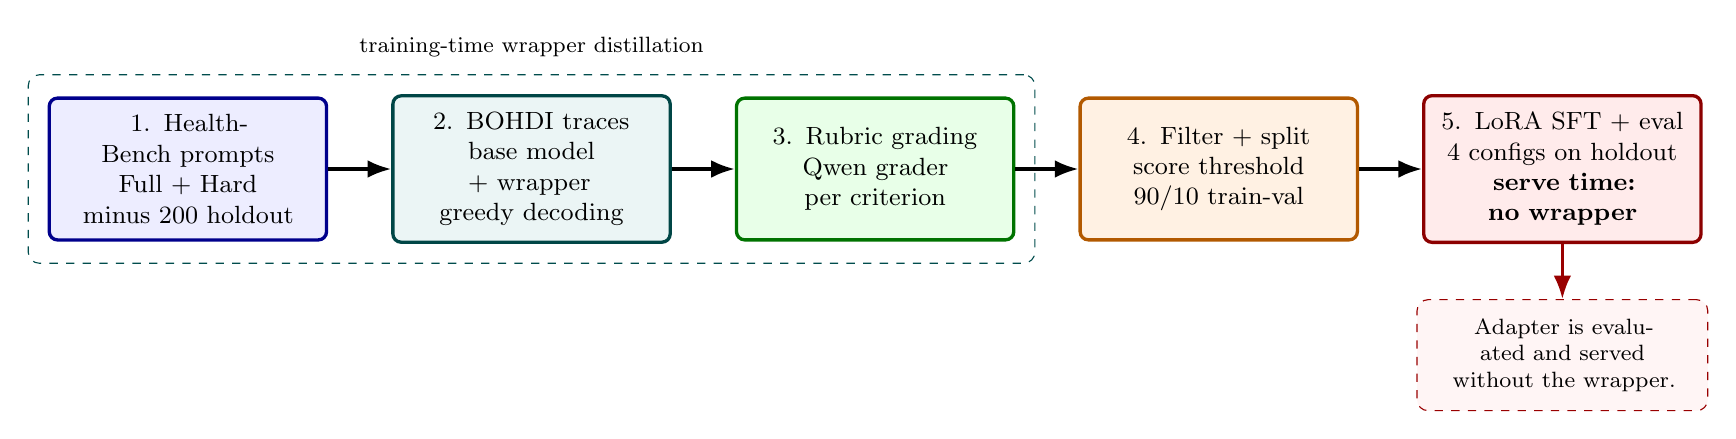
\begin{tikzpicture}[
  font=\small,
  box/.style={
    draw,
    very thick,
    rounded corners=3pt,
    align=center,
    text width=3.1cm,
    minimum height=1.8cm,
    inner sep=6pt,
  },
  flow/.style={-{Latex[length=3mm]}, very thick},
  stage_a/.style={box, draw=blue!55!black, fill=blue!7},
  stage_b/.style={box, draw=teal!55!black, fill=teal!8},
  stage_c/.style={box, draw=green!45!black, fill=green!9},
  stage_d/.style={box, draw=orange!70!black, fill=orange!11},
  stage_e/.style={box, draw=red!55!black, fill=red!8},
  note/.style={
    draw,
    dashed,
    rounded corners=4pt,
    inner sep=7pt,
    align=center,
    font=\footnotesize,
  },
]

\node[stage_a] (prompts) {1. HealthBench prompts\\Full + Hard\\minus 200 holdout};
\node[stage_b, right=8mm of prompts] (wrapper) {2. BOHDI traces\\base model + wrapper\\greedy decoding};
\node[stage_c, right=8mm of wrapper] (grader) {3. Rubric grading\\Qwen grader\\per criterion};
\node[stage_d, right=8mm of grader] (filter) {4. Filter + split\\score threshold\\90/10 train-val};
\node[stage_e, right=8mm of filter] (serve) {5. LoRA SFT + eval\\4 configs on holdout\\\textbf{serve time: no wrapper}};

\draw[flow] (prompts) -- (wrapper);
\draw[flow] (wrapper) -- (grader);
\draw[flow] (grader) -- (filter);
\draw[flow] (filter) -- (serve);

\node[note, draw=teal!60!black, fit=(prompts)(wrapper)(grader)] (train_scope) {};
\node[font=\footnotesize, above=1mm of train_scope] {training-time wrapper distillation};

\node[note, draw=red!60!black, fill=red!4, below=7mm of serve, text width=3.2cm] (serve_note) {Adapter is evaluated and served without the wrapper.};
\draw[flow, red!60!black] (serve.south) -- (serve_note.north);

\end{tikzpicture}
}
  \caption{\textbf{Pipeline overview.} (1) Generate traces on
  HealthBench prompts using a base model wrapped in \textsc{bodhi}.
  (2) Grade each trace against HealthBench's per-criterion rubric using
  a rubric grader model. (3) Filter by score. (4) SFT a LoRA adapter on
  the filtered traces. (5) Evaluate the adapted model
  \emph{without} the wrapper against the base model
  \emph{with} the wrapper, stratified by difficulty tier and theme.}
  \label{fig:pipeline}
\end{figure*}

\subsection{Trace generation}
Given a prompt $x$ from HealthBench, we obtain a wrapper-conditioned
response $y = \textsc{bodhi}(\pi_\text{base}, x)$, where
$\pi_\text{base}$ is MedGemma-27B and the wrapper performs two to five
internal turns of reasoning before emitting $y$. We exclude the 200
prompts reserved for evaluation.

\subsection{Rubric grading}
HealthBench provides a per-prompt rubric: a list of criteria each with a
point value (positive or negative) and descriptive tags. We score each
$(x, y)$ tuple by asking a separate grader model---Qwen-2.5-14B-AWQ for
the paper run, Qwen-2.5-0.5B for cheap iteration---to adjudicate each
criterion~\cite{arora2025healthbench}. The aggregate score for a trace
is $\text{score}(x, y) = \sum_{i \in \text{met}} p_i / \sum_{j: p_j > 0} p_j$,
normalising by the total positive-point budget.

\subsection{Filtering}
We retain only traces with $\text{score}(x, y) \ge 0.4$ and discard
the rest; the threshold was selected by inspecting the score
histogram for a natural break but has not been swept. Retained
traces form the supervision set for the next stage.

\subsection{LoRA fine-tuning}
We fine-tune a low-rank adapter on $\pi_\text{base}$ using the filtered
traces. Default hyperparameters: rank $r{=}16$, $\alpha{=}32$,
dropout $0.05$, target modules
$\{q,k,v,o,\text{gate},\text{up},\text{down}\}_\text{proj}$,
3~epochs, learning rate $10^{-4}$ with cosine decay, warmup ratio $0.05$.
Loss is computed only on the assistant turn via a completion-only
collator. All training is seeded (seed 42) and uses bf16.

\subsection{Stratified evaluation}
\label{sec:eval}
Aggregate accuracy conceals the tails. We report \emph{two
stratifications} in addition to the overall mean:

\paragraph{Difficulty tertiles.} For each prompt, the total
positive-point budget in its rubric is a proxy for difficulty.
We bucket prompts into \textsc{easy}, \textsc{medium}, and \textsc{hard}
by tertile and report mean score and failure rate (score $< 0.4$) per
tier. A flat line across tiers is the goal; an inverted U
indicates the tail-failure pathology.

\paragraph{Per-theme breakdown.}
HealthBench tags each prompt with a theme (e.g.\ \texttt{emergency
referrals}, \texttt{hedging}, \texttt{context seeking}). We report
per-theme failure rates, highlighting \texttt{emergency referrals} and
\texttt{hedging} as the themes where humility-oriented training should
pay off most.

\paragraph{Model-side confidence proxy.}
For calibration-style reporting, we score the emitted response under the
model and compute the geometric mean next-token probability over the
final response tokens. We then report Brier score and ECE against the
positive-point rubric criteria using this response-level confidence
proxy, while retaining the older grader-derived consistency numbers only
for backward comparison in released artifacts.

% =============================================================================
\section{Experiments}
\label{sec:experiments}

\subsection{Setup}
We train four configurations and evaluate on a fixed 200-prompt
HealthBench Hard holdout:
\begin{itemize}[leftmargin=*,topsep=0pt,itemsep=1pt]
\item \textsc{base / no-wrapper} --- MedGemma-27B alone.
\item \textsc{base / bodhi} --- MedGemma-27B + wrapper.
\item \textsc{lora / no-wrapper} --- our headline: LoRA-adapted
      MedGemma-27B, no wrapper at serve time.
\item \textsc{lora / bodhi} --- LoRA-adapted with wrapper
      additionally applied (ceiling-tracking control).
\end{itemize}
All four use greedy decoding. Compute: \tbd{1 H100 hours, total}.

\subsection{Main result}

\begin{table}[t]
  \centering
  \small
  \begin{tabular}{lccc}
    \toprule
    Config & Mean $\uparrow$ & Fail (easy) $\downarrow$ & Fail (hard) $\downarrow$ \\
    \midrule
    Base & \tbd{x} & \tbd{x} & \tbd{x} \\
    Base + Wrapper & \tbd{x} & \tbd{x} & \tbd{x} \\
    LoRA & \tbd{x} & \tbd{x} & \tbd{x} \\
    LoRA + Wrapper & \tbd{x} & \tbd{x} & \tbd{x} \\
    \bottomrule
  \end{tabular}
  \caption{Headline results on 200-prompt HealthBench Hard holdout.
  Mean score is overall; fail rates are stratified by the
  easy/hard tertiles of the per-prompt rubric budget. Lower fail rate
  is better.}
  \label{tab:main}
\end{table}

\tbd{Prose interpretation. Headline claim if validated:
\textsc{lora / no-wrapper} matches or exceeds
\textsc{base / bodhi} on the mean and---critically---on both tails,
supporting the weight-level internalization hypothesis. Honest
caveats in the other direction go in \S\ref{sec:limitations}.}

\subsection{U-shape analysis}

\begin{figure}[t]
  \centering
  \includegraphics[width=\linewidth]{figures/u_fail_smooth.pdf}
  \caption{\textbf{Failure rate vs.\ rubric difficulty.} Points are
  equal-frequency bin means (10 bins); curves are quadratic fits.
  \tbd{Real caption: the inverted-U is pronounced for the base
  model and flattens on the LoRA-adapted model, with wrapper conferring
  an additional margin on the hardest tier.}}
  \label{fig:ushape}
\end{figure}

\subsection{Per-theme}

\begin{figure}[t]
  \centering
  \includegraphics[width=\linewidth]{figures/theme_fail.pdf}
  \caption{\textbf{Per-theme failure rate.}
  \texttt{emergency\_referrals} and \texttt{hedging} are highlighted
  as the themes where humility-oriented training should produce the
  largest drop. \tbd{Actual magnitude.}}
  \label{fig:themes}
\end{figure}

\subsection{Ablation on a smaller base}
To check whether the effect is specific to MedGemma-27B's scale, we
repeat the pipeline with Gemma-3n-E4B as the base. \tbd{Whether the U
also flattens at 4B, or whether the behaviour requires the larger
model's capacity.}

% =============================================================================
\section{Limitations and Open Choices}
\label{sec:limitations}

We flag three methodological decisions that affect the strength of any
claim and that this workshop paper does not yet resolve:

\textbf{Grader coupling.} The same grader is used for both training-data
filtering and final evaluation. A model that succeeds by matching the
grader's biases rather than producing genuinely correct answers would be
rewarded. A second-grader cross-check is an obvious remedy and is
deferred to the full-length version.

\textbf{Calibration metric semantics.} Even after moving off the
grader's aggregate score, our confidence signal is still only a
response-level logprob proxy, not a dedicated uncertainty head or an
explicit abstention probability. We therefore treat Brier score and ECE
as calibration-style evidence rather than a complete account of model
uncertainty, and keep the older \texttt{*\_grader\_consistency} fields
only for backward comparison.

\textbf{Score normalisation.} Our aggregation
$\sum_\text{met} p_i / \sum_{p_j > 0} p_j$ permits negative total
scores when penalty criteria fire, which interacts awkwardly with the
threshold-based filter. A principled alternative
(e.g.\ $\sum_\text{met} p_i / \sum |p_j|$ or per-prompt z-score) is
left to future work.

\textbf{Scope.} Single seed, single test split. Variance bars are
absent. Only text-only HealthBench Hard; real clinical deployment
would demand broader coverage.

% =============================================================================
\section{Conclusion}

We sketched a pipeline for distilling an epistemic wrapper's behaviour
into a model's weights via LoRA fine-tuning, and argued that a stratified
evaluation is needed to tell whether the distillation actually buys
what we care about. \tbd{One-sentence summary of the result if it
holds.} The proposal, pipeline, and anonymized code are available now;
the full paper-scale run will be released with the non-anonymous
version.

% =============================================================================
\section*{Impact Statement}
Clinical LLM deployment tolerates mistakes poorly. Methods that make
models \emph{quieter} about what they don't know---especially on
emergency-referral and hedging-required cases---plausibly reduce harm
rather than cause it. The risk we are most aware of is that an
internalized humility signal could be over-generalised, making the
model refuse legitimate requests; the per-theme and per-tier breakdowns
in \S\ref{sec:eval} are designed to detect this.

% =============================================================================
\bibliography{references}
\bibliographystyle{icml2026}

\end{document}
